\section{Biofilm as a virulence factor produced by \textit{P. aeruginosa}}

The biofilm \textit{P. aeruginosa} excretes, contains specific polysaccharides as well as protein and eDNA. The biofilm formation increases the bacteria's pathogenicity by blocking the antibiotics from reaching the bacteria \cite{Thi2020PseudomonasBiofilms}. Generally biofilm can be produced both by a single bacterial species as well as by a mixture of species. This can further increase the complexity of biofilms. 

Before production of biofilm, \textit{P. aeruginosa} uses the flagella for motility in the plaktonic state until it reaches a desired surface. The construction of this flagella in \textit{P. aeruginosa} is zinc dependent due to the Zur-locus \cite{Mastropasqua2018EfficientLung}. The Zur-locus is a regulatory transcription gen, consisting of \textit{zrmA}, \textit{dksA2} and \textit{rpmE2}. When \textit{P. aeruginosa} is exposed to low levels of zinc, there is a higher expression of this locus \cite{Mastropasqua2018EfficientLung}. The genes in the Zur-locus have been related to the interference and formation of biofilm, due to the zinc dependent flagella. \textit{P. aeruginosa}'s swarming and flagella are dependent on zinc concentration. Therefore, zinc is a key player in the pre-stage of biofilm production \cite{Mastropasqua2018EfficientLung}.

\subsection{Biofilm formation} 
\noindent When biofilm is initiated, planktonic bacteria adhere to a surface which is often nutrient rich and favorable for bacterial growth. In \textit{P. aeruginosa} the attachment is mediated by the flagella or pili \cite{Ma2009AssemblyMatrix}. After adhesion the flagella and pili functions are reduced. The next stage of the biofilm formation is colonization. 
During colonization the bacteria multiply and start to produce sticky extracellular polymer substances (EPS). Throughout development the bacteria in the biofilm begin to change their metabolism which can result in complex systems. In these complex systems the bacteria at the top of the biofilm can be different from those at the base. Further the complex systems in \textit{P. aeruginosa} biofilm can take form of mushroomlike columns and channels. Finally the mature biofilm disperses allowing the detached bacteria to colonize to new locations \cite{Ma2009AssemblyMatrix} (figure \ref{fig:biofilm}). \\

\begin{figure}[H]
    \centering
    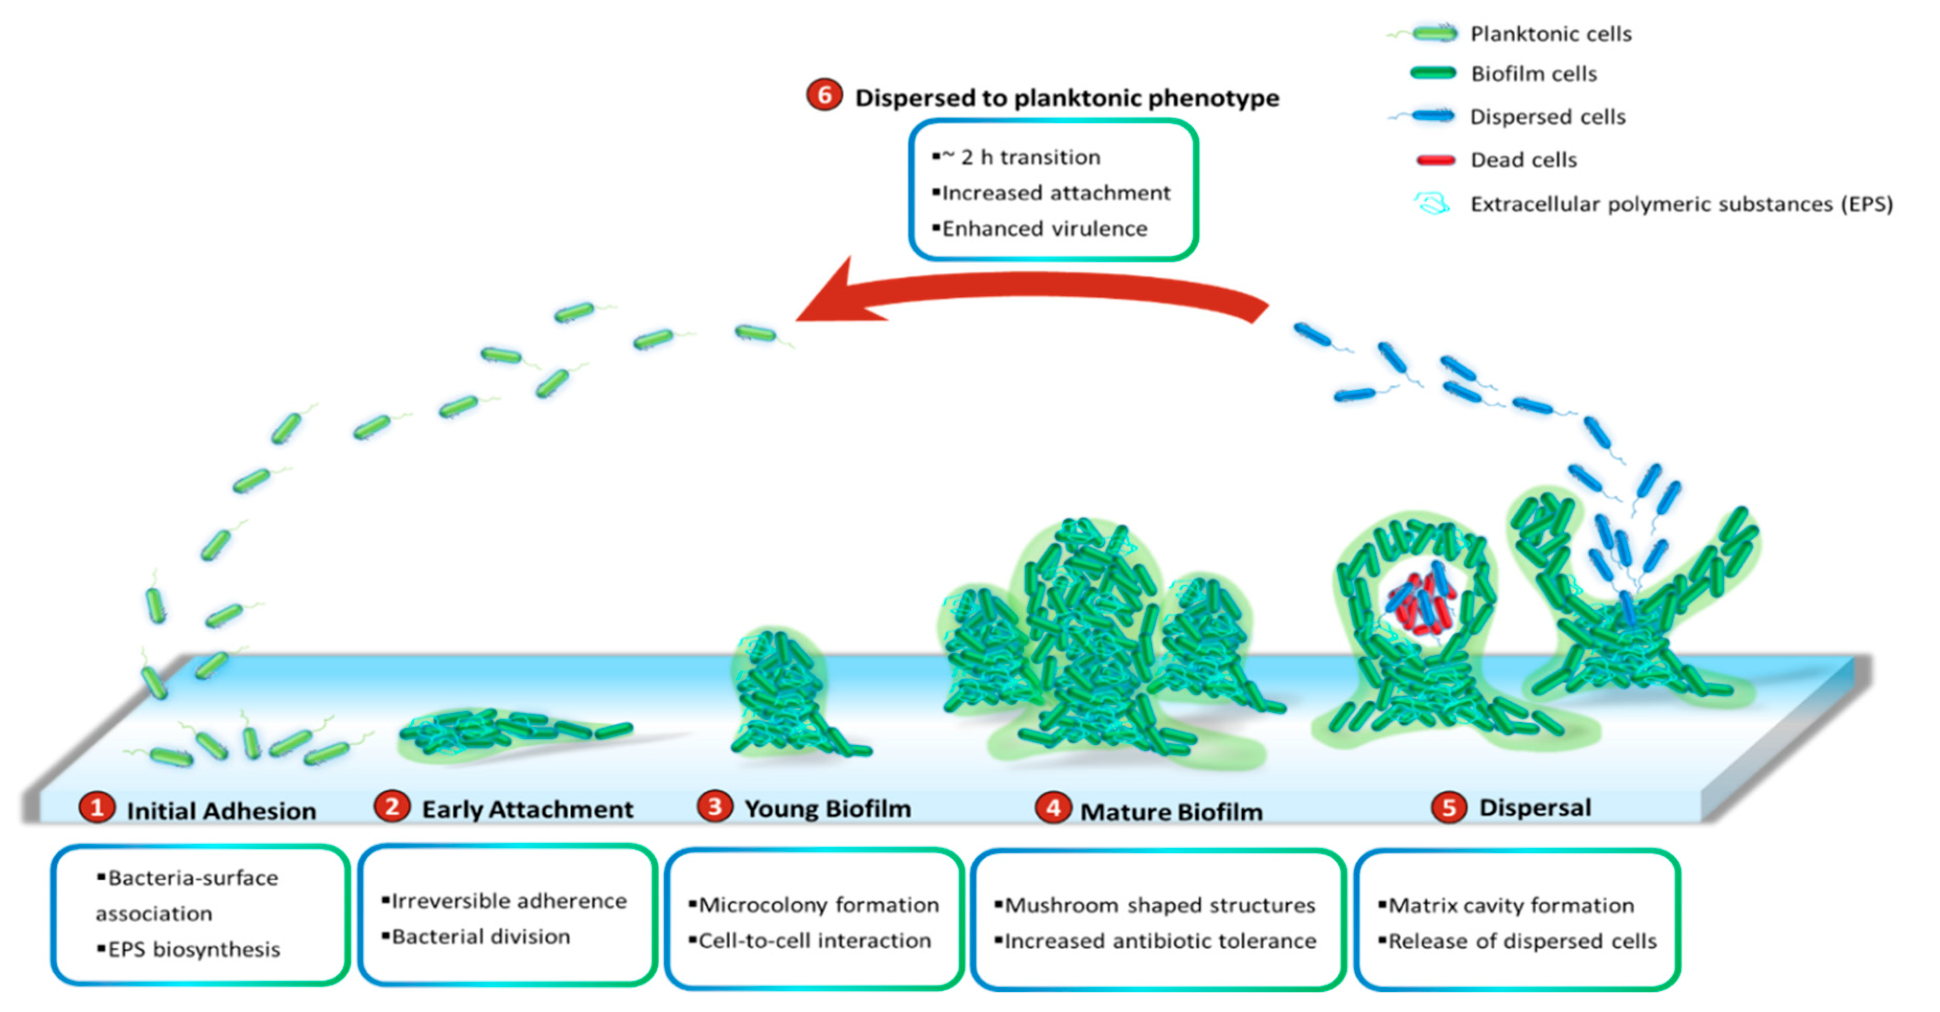
\includegraphics[width=\textwidth]{Figures/Screenshot 2022-04-27 at 10.00.54.png}
    \caption{\footnotesize{The cycle of \textit{P. aeruginosa} biofilm formation. The cycle is divided into six stages. The first step is initial adhesion, followed by early attachment. During these first stages the bacteria begin to produce extracellular polymeric substances followed by cell division. The following steps are the formation of microcolonies and the further development of these microcolonies into mushroom-shaped structures. Finally the mature biofilm disperses bacteria which allows for new colonization sites \cite{Thi2020PseudomonasBiofilms}.}}
    \label{fig:biofilm}
\end{figure}

\subsection{Quorum sensing as a factor in biofilm formation}

\noindent Inside the biofilm, nutrients can fluctuate between the bacteria. Further the matrix creates an environment for natural transformation and gen exchange, as well as resistance against the outside environment \cite{Madigan2022BrockMicroorganisms}. Bacteria inside the biofilm are tightly packed, which allows cell-to-cell communication called quorum sensing (QS). The phenomenon of QS is mainly found among gram-negative bacteria, and it works through regulatory molecules called autoinducers. Autoinducers can diffuse and be absorbed between bacteria within the biofilm. Specifically for \textit{P. aeruginosa}, high expression of the autoinducer acyl homoserine lactones (AHL), binds and activates transcriptional proteins \cite{Madigan2022BrockMicroorganisms}. The formation of biofilm is controlled by autoinducers as well as the concentration of secondary messengers, such as cyclic di-guanosine monophosphate (c-di-GMP). \\

\noindent When the population of \textit{P. aeruginosa} reaches a high enough concentration of AHL, secondary messengers related to biofilm formation can be expressed. One of these is secondary messengers is c-di-GMP. An increase in c-di-GMP levels cause weakend function of the flagellum as well as the fabrication of EPSs \cite{Colvin2012TheMatrix} \cite{Madigan2022BrockMicroorganisms}. Part of these EPSs is the pentasaccharide Psl which shields the biofilm bacteria from antimicrobials \cite{Billings2013TheBiofilms}. Additionally Psl functions as a signaling molecule for the production of c-di-GMP. Elevated c-di-GMP levels also creates a thicker and more robust biofilm \cite{Irie2012Self-producedAeruginosa/i}. Furthermore lysed cells excrete DNA that can also contribute to the biofilm formation.\\

\noindent Biofilm is a major problem for patients with cystic fibrosis as the matrix makes it difficult to treat. During hypoxic and anoxic conditions \textit{P. aeruginosa} has indicated the ability to grow slowly as unattached cell aggregates, reviewed in Thi \textit{et. al.} \cite{Thi2020PseudomonasBiofilms}. Slowly growing biofilms with limited oxygen are ascribed to antibiotic recalcitrance \cite{Thi2020PseudomonasBiofilms}. Still to this day, there hasn't been found an effective treatment to fight the invasion of biofilm, when infected with \textit{P. aeruginosa}. Alternative treatment options to antibiotics will be discussed in the following section. 



